\documentclass{report}

\usepackage[utf8]{inputenc}
\usepackage{polski}

\usepackage{graphicx}
\usepackage{tabularx}

%do edytowania marginesów
\usepackage{changepage}

%Do edytowania list
\usepackage{enumitem}
\setitemize[1]{label={--}}

\title{"Terraria \ppauza poradnik w poczatkowych fazach gry"}
\author{Cezary Kwella}

\begin{document}
\maketitle
\tableofcontents
\listoftables
\chapter*{Wstęp}
\addcontentsline{toc}{chapter}{Wstęp}
\paragraph{} W niniejszym krótkim poradniku chciałbym wyjaśnić podstawowe aspekty gry ,,Terraria'' studia \textbf{Re-Logic}.
\chapter{Początki}
\section{Rozpoczęcie nowej gry}
\subsection{Tryb gry} 
\paragraph{} W menu po włączeniu gry ukaże nam się wybór \textit{trybu gry}. Mamy do wyboru tryb jedno\dywiz i wieloosobowy. Jak sama nazwa wskazuje, od tego zależy, czy będziemy grać sami, czy z innymi \ppauza np. poprzez serwery \textit{steama}.
\subsection{Tworzenie postaci}
\paragraph{} Po wybraniu trybu gry, ukaże nam się okno kreatora postaci. Znajdziemy tutaj następujące opcje:
\begin{itemize}
\item \textbf{wygląd postaci},
\item \textbf{nazwa},
\item \textbf{poziom trudności postaci} \ppauza różnice przedstawiono na  \textbf{tabeli \ref{tab:difficulty}}.
	\begin{table}
	\centering
	\begin{adjustwidth}{-2.4cm}{}
	\begin{tabular}{|p{0.25\linewidth}|p{0.25\linewidth}|p{0.25\linewidth}|p{0.25\linewidth}|}
	\hline
	\textbf{podróż} & \textbf{klasyczny} & \textbf{średni} & \textbf{hardcore} \\
	\hline
	\begin{itemize}
	\item Postać rozpoczyna grę z dodatkowym wyposażeniem,
	\item głównie do testowania,
	\item możliwość cheatowania. 
	\end{itemize} &
	\begin{itemize}
	\item Po śmierci postacie upuszczają tylko (albo i aż) zdobyte pieniądze, 
	\item \textbf{polecany} podczas pierwszej rozgrywki. 
	\end{itemize} & 
	\begin{itemize}
	\item Oprócz pieniędzy po śmierci upuszczane są wszystkie posiadane w ekwipunku przedmioty.
	\end{itemize} & 
	\begin{itemize}
	\item Po śmierci na tym poziomie nie można się odrodzić,
	\item \textbf{wyzwanie} dla bardzo zaawansowanych graczy.
	\end{itemize} \\
	\hline
	\end{tabular}
	\end{adjustwidth}
	\caption{Porownanie trybów trudności gry}
	\label{tab:difficulty}
	\end{table}
\end{itemize}
\subsection{Tworzenie świata}
\paragraph{} Po stworzeniu postaci otworzy nam się nowe okno - kreator świata. 
\begin{figure}
	\centering
	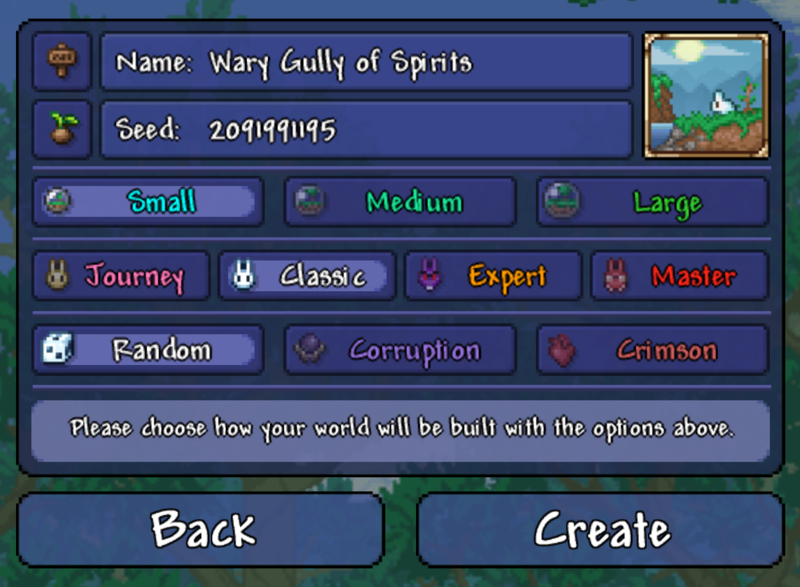
\includegraphics[scale=0.4]{createWorld}
	\caption{Przykładowe menu tworzenia świata w języku angielskim}
	\label{rys:world}
\end{figure}
Na \textbf{rysunku \ref{rys:world}} widać opcje, które możemy ustawić. Są to: 
\begin{itemize}
	\item nazwa,
	\item ziarno generatora,
	\item rozmiar świata,
	\item poziom trudności świata,
	\item rodzaj złego biomu (polecany \textbf{losowy}).
\end{itemize}
\paragraph{} Po wybraniu wszystkich opcji, jeśli jesteśmy gotowi na przygodę wybieramy \textit{Stwórz} oraz rozpoczynamy grę!
\chapter{Pierwsze dni}
\end{document}